\section{Methods}
\label{sec:methods}

\subsection{Terrain}

The terrain comes from the Amazon Web Services (AWS) Terrain Tiles, a digital elevation
model (DEM) with a grid spacing of about \SI{\nDEMres}{\meter}.
Slope and aspect (the direction a slope faces) are computed within
\SI{\nSlopeRadius}{\meter} of the abbey, along with a southwest--northeast elevation section.
The grid smooths the steep edge of the spur, so slopes are lower bounds.

\begin{figure}[htbp]
  \centering
  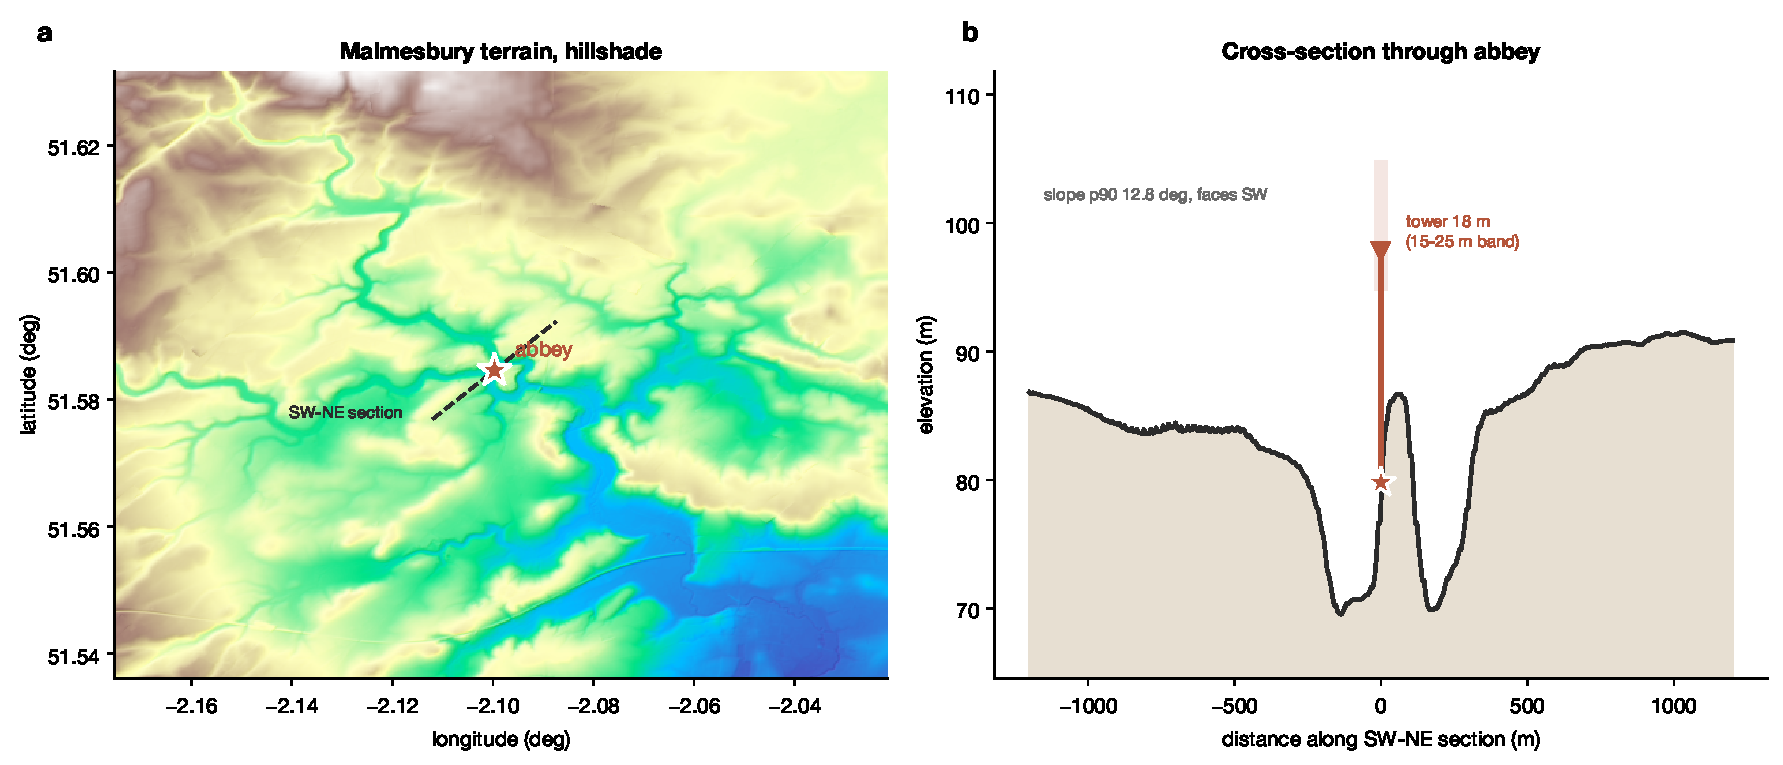
\includegraphics[width=\linewidth]{fig1_site}
  \caption{\textbf{Terrain at Malmesbury Abbey.}
  \textbf{(a)} Hillshaded DEM (AWS Terrain Tiles); the dashed line is the section in (c).
  \textbf{(b)} Southwest-facing ground steeper than \ang{\nSWFaceSlope} within \SI{\nSitePanel}{\meter} of the
  abbey (star), in orange.
  The green line is the track along the slope (\SI{\nLiftAlongSlope}{\meter}); the grey
  arrow is the first \SI{\nTarget}{\meter} of the track into the wind.
  \textbf{(c)} Elevation along the section, with the sampled tower heights.}
  \label{fig:site}
\end{figure}

\subsection{Wind climatology}

Hourly \SI{10}{\meter} wind at the abbey for 2004--2023 (\nHours\ hours) comes
from the ERA5 reanalysis of the European Centre for Medium-Range Weather Forecasts
\autocite{hersbach2020era5}, through the Open-Meteo archive
\autocite{openmeteo_archive}.
An hour is favourable when the wind blows from the southwest sector
(\ang{\nSectorLo}--\ang{\nSectorHi}, centred on the slope aspect) at \SIrange{\nSpeedLo}{\nSpeedHi}{\meter\per\second}.
Annual and seasonal fractions have \SI{95}{\percent} confidence intervals (CI) across the
twenty years.
Modern data stand in for the eleventh century.
Reconstructions of the North Atlantic Oscillation (NAO), the pressure pattern that sets the
strength of the westerlies over Britain, disagree on its medieval phase
\autocite{trouet2009nao,ortega2015nao}.
Neither indicates a long negative phase with weak westerlies.

\subsection{Ridge lift}

Wind blowing up a slope is deflected upwards, with a vertical velocity that to first order
follows the surface gradient and decays with height,
\begin{equation}
  w(x,z) = U\,\frac{\mathrm{d}h}{\mathrm{d}x}\,e^{-kz},
  \label{eq:ridge}
\end{equation}
where \(U\) is the wind speed, \(h(x)\) the terrain height along the wind, \(z\) the height
above the surface, and \(k = 2\pi/L\) with \(L\) the horizontal scale of the slope.
Supplementary \cref{fig:ridge} applies \cref{eq:ridge} to the measured section; the glide
model uses the simpler surface estimate \(w = \eta\,U\sin\theta_s\), where
\(\theta_s\) is the slope angle and \(\eta \le 1\) allows for flow that does not follow the
surface.
This lift extends \SI{\nLiftIntoWind}{\meter} on the track into the wind and
\SI{\nLiftAlongSlope}{\meter} on the track along the slope (\cref{fig:site}b).

\subsection{Glide performance}

The glide ratio \LD\ of an unknown wing follows from the parabolic drag polar
\(C_D = C_{D0} + C_L^2/(\pi e A)\), whose maximum is
\begin{equation}
  (\LD)_\mathrm{max} = \frac{1}{2}\sqrt{\frac{\pi e A}{C_{D0}}},
  \label{eq:polar}
\end{equation}
where \(A\) is the aspect ratio (span squared over area), \(e\) the span efficiency, and
\(C_{D0}\) the zero-lift drag coefficient \autocite{drela2014flight}.
An aspect ratio of \numrange{\nARlo}{\nARhi} gives a span of one to two arm spans for areas
of \SIrange{\nAreaLo}{\nAreaHi}{\meter\squared}.
Span efficiencies of \numrange{\nElo}{\nEhi} cover untwisted, non-elliptical wings
\autocite{drela2014flight}.
The zero-lift drag \(C_{D0} = \numrange{\nCDzlo}{\nCDzhi}\) adds the profile drag of a
cambered membrane at a Reynolds number near \num{e\nReExp}
\autocite{lissaman1983lowre,hoerner1985lift} to the drag of the pilot's body, frame and
bracing \autocite{hoerner1965drag}.
These ranges give \((\LD)_\mathrm{max} = \numrange{\nLDlo}{\nLDhi}\), with \num{\nLDnom}
at their centres.
Every wing is flown at its best glide ratio, which favours the account.

A wing of area \(S\) carrying mass \(m\) at lift coefficient \(C_L\) trims at
\(V = \sqrt{2mg/(\rho S C_L)}\), \SI{\nTrimSpeed}{\meter\per\second} for the nominal
configuration of \cref{fig:apparatus} (\SI{\nMass}{\kilogram}, \SI{\nArea}{\meter\squared},
\(C_L = \nCLtrim\)).

\begin{figure}[htbp]
  \centering
  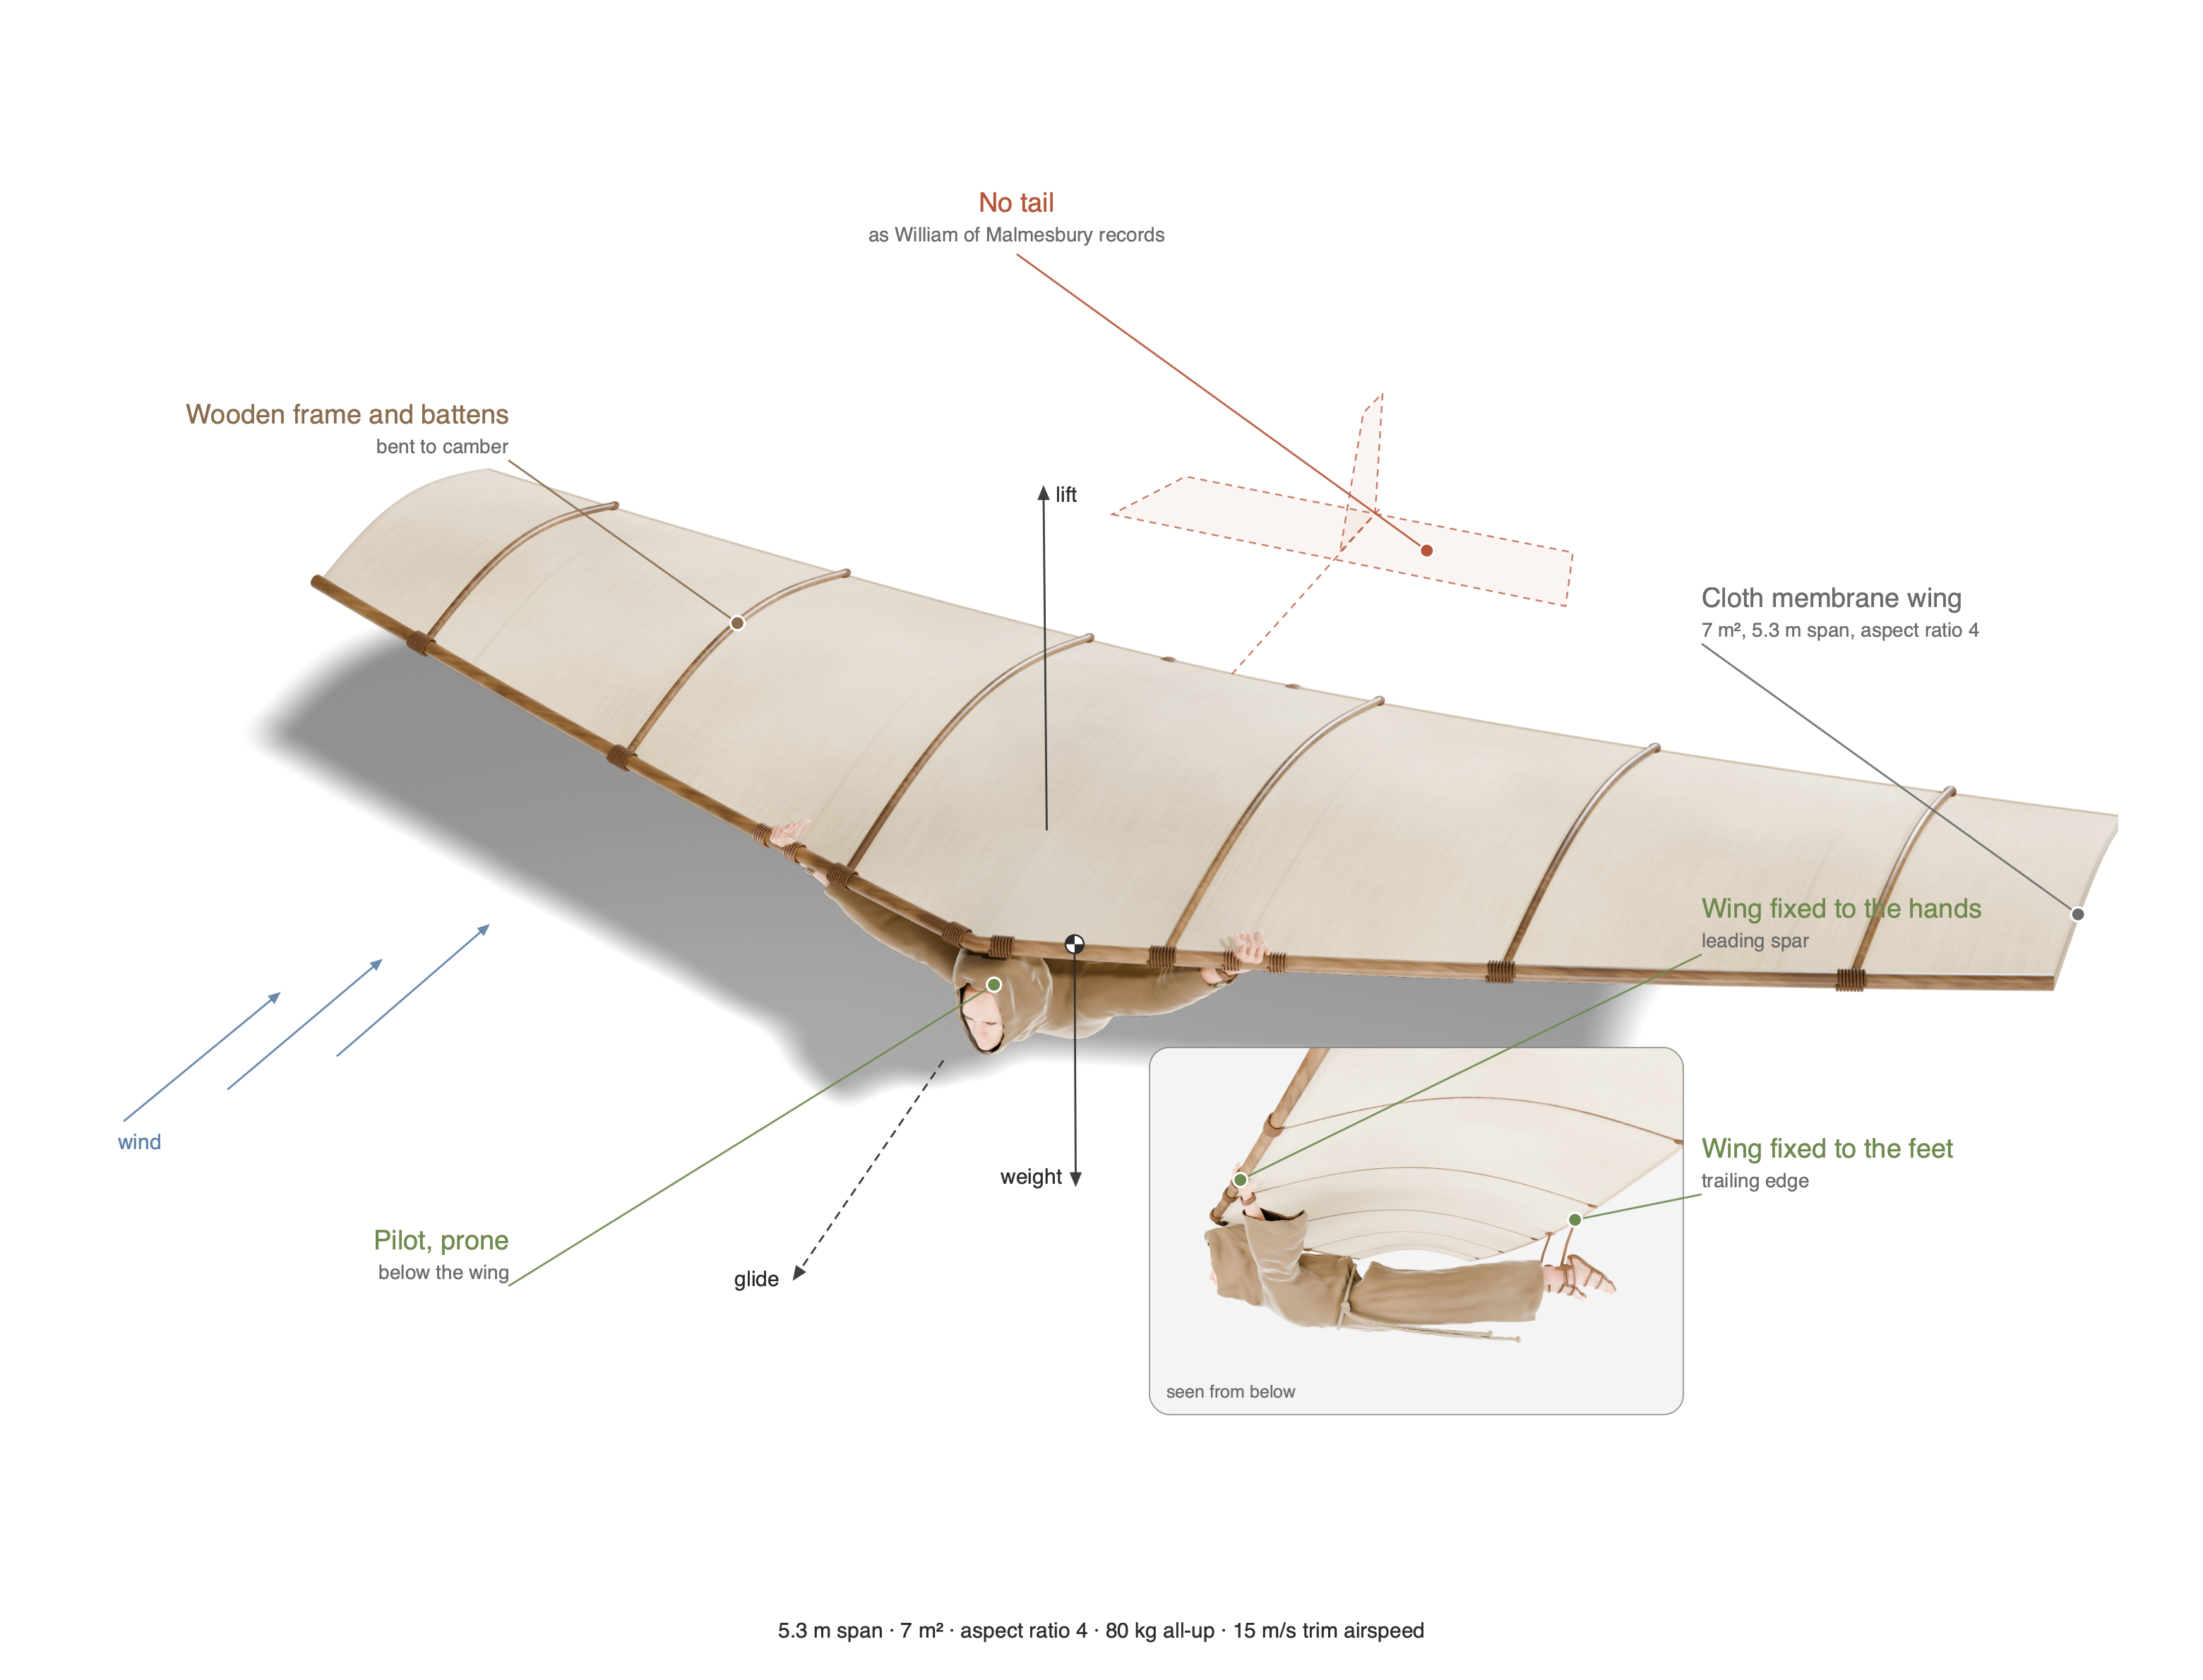
\includegraphics[width=0.75\linewidth]{fig_apparatus}
  \caption{\textbf{Nominal model configuration, not a reconstruction.}
  A tailless cloth wing fixed to the prone pilot's hands (leading edge) and feet (trailing
  edge).
  Only the attachment and the missing tail come from the source; the dimensions are the centres of the sampled
  ranges (Supplementary \cref{tab:priors}).
  The dashed outline marks where a tail would be; arrows show lift, weight, glide and headwind.}
  \label{fig:apparatus}
\end{figure}

\subsection{Launch and glide trajectory}

A man stepping off a tower leaves at about \SI{\nJump}{\meter\per\second} relative to the
ground and dives until the airspeed reaches \(V\), so the flight is integrated as a point mass at constant
\(C_L\),
\begin{equation}
  \dot V = g\sin\gamma - \frac{D}{m}, \qquad
  \dot\gamma = \frac{1}{V}\left(g\cos\gamma - \frac{L}{m}\right), \qquad
  \dot z = -V\sin\gamma + w,
  \label{eq:eom}
\end{equation}
where \(V\) is now the airspeed, \(\gamma\) the descent angle below the horizontal,
\(L = \frac{1}{2}\rho V^2 S C_L\), and \(D = L/(\LD)\).
The airspeed at release is the jump speed plus the headwind.

Two tracks bracket the ground covered.
On the first, the pilot heads southwest into the wind, down the slope towards the river
\autocite{woosnam1986eilmer}, at ground speed \(V\cos\gamma - U\) over the measured section.
On the second, he flies northwest along the slope with the wind from the side, as
hang-glider and sailplane pilots use ridge lift \autocite{faa_glider}.
He crabs, heading partly into the wind to hold the track, at ground speed
\(\sqrt{(V\cos\gamma)^2 - U^2}\) over a contour \SI{\nContour}{\meter} below the abbey.
William's ``more than a furlong'' becomes a ground range of at least \SI{\nTarget}{\meter}.

\subsection{Pitch stability}

A wing is stable in pitch if the centre of gravity (CG) lies ahead of the
neutral point, about which the pitching moment does not change with angle of attack.
Both are measured from the leading edge as fractions of the mean chord \(c\), \(\cgfrac\)
and \(\npfrac\).
A cambered wing without a tail has \(\npfrac \approx \nNPnotail\); a tail moves it aft, to
\num{\nNPtail} for the nominal tail, and adds pitch damping \autocite{drela2014flight}.

The pilot's mass centre lies between his hands, at the leading edge, and feet, at the
trailing edge.
Standing, it is at about \SI{\nComHeightPct}{\percent} of his height above the soles
\autocite{winter2009biomechanics}, and his reach from soles to raised hands is about
\num{\nReachRatio} times his height.
Laid out, it lies about \num{\nCGstraight} of the hand-to-foot distance behind the hands.
The sampled range \(\cgfrac = \numrange{\nCGlo}{\nCGhi}\) runs from this straight posture
forward to hips drawn up under the leading edge.
A wider sweep, \(\cgfrac = \numrange{\nCGsweepLo}{\nCGsweepHi}\), shows where the conclusion would change.

With the CG aft of the neutral point, the short-period motion, linearised in angle of attack
and pitch rate \autocite{drela2014flight}, has a positive real eigenvalue \(\lambda\), so a
disturbance doubles in \(t_2 = \ln 2/\lambda\).
\(t_2\) is compared with the flight time and a human operator's effective
time delay in manual control, about \SIrange{\nReactLo}{\nReactHi}{\second}
\autocite{mcruer1967pilot}.
A nonlinear run tests an \ang{\nGust} gust, with control lost beyond \ang{\nPitchLoss} of pitch.

\subsection{Monte Carlo sample}

Because the apparatus and the day are unknown, \nSamples\ cases are drawn with a fixed
seed from the uniform ranges of every parameter above (Supplementary
\cref{tab:priors}), except the glide ratio, which follows from \cref{eq:polar}.
The launch wind is drawn from the ERA5 southwest-sector hours at
\SIrange{\nWindLo}{\nWindHi}{\meter\per\second}, assuming Eilmer chose a windy day.
Each case is flown on both tracks with \cref{eq:eom} and scored on whether it covers
\SI{\nTarget}{\meter} and whether \(t_2\) is shorter than the flight, with and without a tail.
Fractions have Wilson score \SI{95}{\percent} CIs.

\subsection{Impact}

William records that Eilmer broke both legs and survived.
In a feet-first landing the body stops over a distance \(d\) of leg flexion and ground
give, so a vertical arrival speed \(v\) gives a mean force
\begin{equation}
  F = \frac{m v^2}{2 d}, \qquad \text{shared between two legs.}
  \label{eq:impact}
\end{equation}
The tibia breaks under axial and combined loads of \SIrange{\nTibiaLo}{\nTibiaHi}{\kilo\newton}
per leg \autocite{salzar2014leg,abidin2026tibia,forman2012femur,ivarsson2005bending,femurFE2022},
which sets a fracture-onset speed \(v^\star = \sqrt{2 d F_\mathrm{tot}/m}\) for
\(d = \SIrange{\nStopLo}{\nStopHi}{\centi\meter}\).
Two arrivals are compared for cases that reach \SI{\nTarget}{\meter}.
A controlled glide without a flare meets the ground at the vertical speed from
\cref{eq:eom}.
After a loss of pitch control the craft strikes at airspeed \(V\) along a path
\ang{\nDepAngLo}--\ang{\nDepAngHi} below horizontal, with vertical speed \(V\sin\theta\).
Because \cref{eq:impact} uses the mean force, peak loads are higher and the onset speeds are
upper bounds.
